\documentclass[a4paper, 12pt]{article}

\usepackage{hyperref}
\usepackage[warn]{mathtext}
\usepackage[utf8]{inputenc}
\usepackage[T2A]{fontenc}
\usepackage[english,russian]{babel}
\usepackage{multirow}
\usepackage{float}
\restylefloat{table}
\usepackage{amsmath,amsfonts,amssymb,amsthm,mathtools}
\usepackage{indentfirst}
\DeclareSymbolFont{T2Aletters}{T2A}{cmr}{m}{it}
\usepackage{ gensymb }
\mathtoolsset{showonlyrefs=true}
\usepackage{euscript}
\usepackage{mathrsfs}
\usepackage[left=2cm,right=2cm,top=2cm,bottom=2cm]{geometry}
\usepackage{graphicx}
\usepackage{wrapfig}
\usepackage[rgb]{xcolor}
\hypersetup{
colorlinks=true,
urlcolor=blue
}
\usepackage{tikz}

\title{Лабораторная работа}
\author{Гисич Арсений Б03-101}
\date{2023}

\begin{document}

	\begin{center}
		{\large МОСКОВСКИЙ ФИЗИКО-ТЕХНИЧЕСКИЙ ИНСТИТУТ (НАЦИОНАЛЬНЫЙ ИССЛЕДОВАТЕЛЬСКИЙ УНИВЕРСИТЕТ)}
	\end{center}
	\vspace{5 cm}
	{\Large
		\begin{center}
			{\bf Лабораторная работа 5.1.1}\\[0.2 cm]
			Экспериментальная проверка уравнения Эйнштейна для фотоэффекта и определение постоянной Планка
		\end{center}
	}
	\vspace{4 cm}
	\begin{flushright}
		{\Large Выполнили: \\
			\vspace{0.2 cm}
			Гисич Арсений \\
            Вазюля Василиса \\ 
			\vspace{0.2 cm}
			Б03-101 \\}
	\end{flushright}
	\vspace{7 cm}
	\begin{center}
		Долгопрудный\\[0.1 cm]
		2023
	\end{center}
\thispagestyle{empty}

\section{Аннотация}

В данной работе исследовалась зависимость фототока от величины задерживающего потенциала и частоты падающего излучения, что позволяет вычислить величину постоянной Планка.

\section{Теоретические сведения}

Фотоэффект --- явление испускания электронов фотокатодом, облучаемым светом,  Это явление хорошо объясняется фотонной теорией света. Взаимодействие монохроматического света с веществом можно описывать
	как взаимодействие с веществом частиц, называемых фотонами, которые обладают энергией $ \hbar \omega $ и импульсом $ \hbar\omega/c $. При столкновении фотона с электроном фотокатода энергия отона полностью передается электрону, и фотон прекращает свое существование. Энергетический баланс этого взаимодействия для вылетающих электронов
	описывается уравнением
	
	\begin{equation}\label{energy balance}
	\hbar \omega = E_{max} + W
	\end{equation}
	
	\begin{wrapfigure}{l}{0.3\linewidth}
		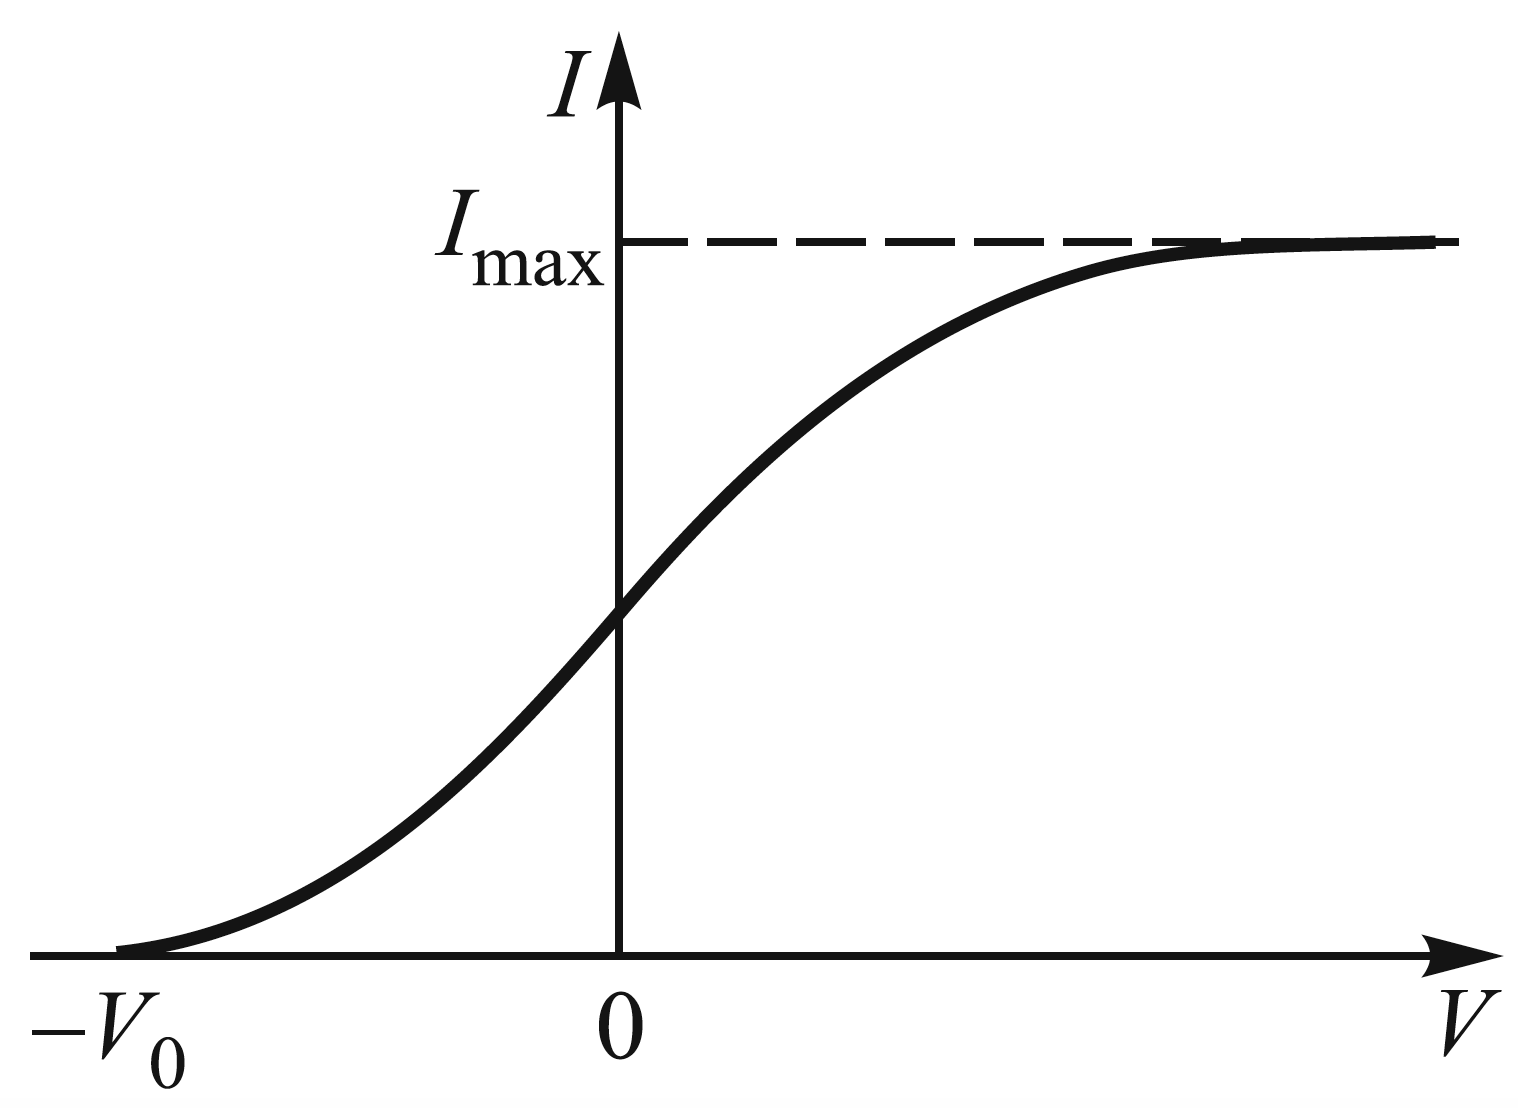
\includegraphics[width=\linewidth]{I(V)}
		\caption{Зависимость фототока от напряжения на аноде фотоэлемента}
		\label{ris I(V)}
	\end{wrapfigure}
	
	Здесь $ E_{max} $ ---  максимальная кинетическая энергия электрона после выхода из фотокатода, $ W $ --- работа выхода электрона из катода. Реально энергетический спектр вылетевших из фотокатода электронов непрерывен --- он простирается от нуля до $ E_{max} $. 
	
	Для измерения энергии вылетевших фотоэлектронов вблизи фотокатода
	обычно располагается второй электрод
	(анод), на который подается задерживающий ($ V < 0 $) или ускоряющий ($ V >
	0 $) потенциал. При достаточно больших
	ускоряющих напряжениях фототок достигает насыщения (рис. \ref{ris I(V)}): все испущенные электроны попадают на анод.
	
	При задерживающих потенциалах на анод попадают лишь электроны,
	обладающие достаточно большой кинетической энергией, в то время
	как медленно движущиеся электроны заворачиваются полем и возвращаются на катод. При некотором значении $ V = -V_0 $ (потенциал запирания) даже наиболее быстрые фотоэлектроны не могут достичь
	анода.
	Максимальная кинетическая энергия $ E_{max} $ электронов связана с
	запирающим потенциалом $ V_0 $ очевидным соотношением $ E_{max} = eV_0 $. Тогда \eqref{energy balance} примет вид, называемый уравнением Эйнштейна:
	
	\begin{equation}\label{Einsteain}
	eV_0 = \hbar\omega - W 
	\end{equation}
	
	Чтобы определить величину запирающего
	напряжения, нам надо правильно экстраполировать получаемую токовую зависимость к нулю, т. е. определить, какова функциональная
	зависимость $ I(V) $. Расчет для простейшей геометрии --- плоский катод, освещаемый светом, и параллельный ему анод --- приводит к зависимости
	
	\begin{equation}\label{sqrt I = V}
	\sqrt{I} \propto V_0 - V
	\end{equation}
	
	т. е. корень квадратный из фототока линейно
	зависит от запирающего напряжения. Эта зависимость хорошо описывает экспериментальные данные.
	
	В работе изучается зависимость фототока из фотоэлемента от величины задерживающего потенциала $ V $ для различных частот света $ \omega $, лежащих в видимой области спектра. С целью экспериментальной
	проверки уравнения Эйнштейна определяются потенциалы запирания
	$ V_0 $ при разных частотах света и строится зависимость $ V_0(\omega) $, которая, как это следует из \eqref{Einsteain}, должна иметь вид
	
	\begin{equation}\label{V(w)}
	V_0 (\omega) = \dfrac{\hbar\omega - W}{e}
	\end{equation}
	
		\begin{wrapfigure}{r}{0.3\linewidth}
		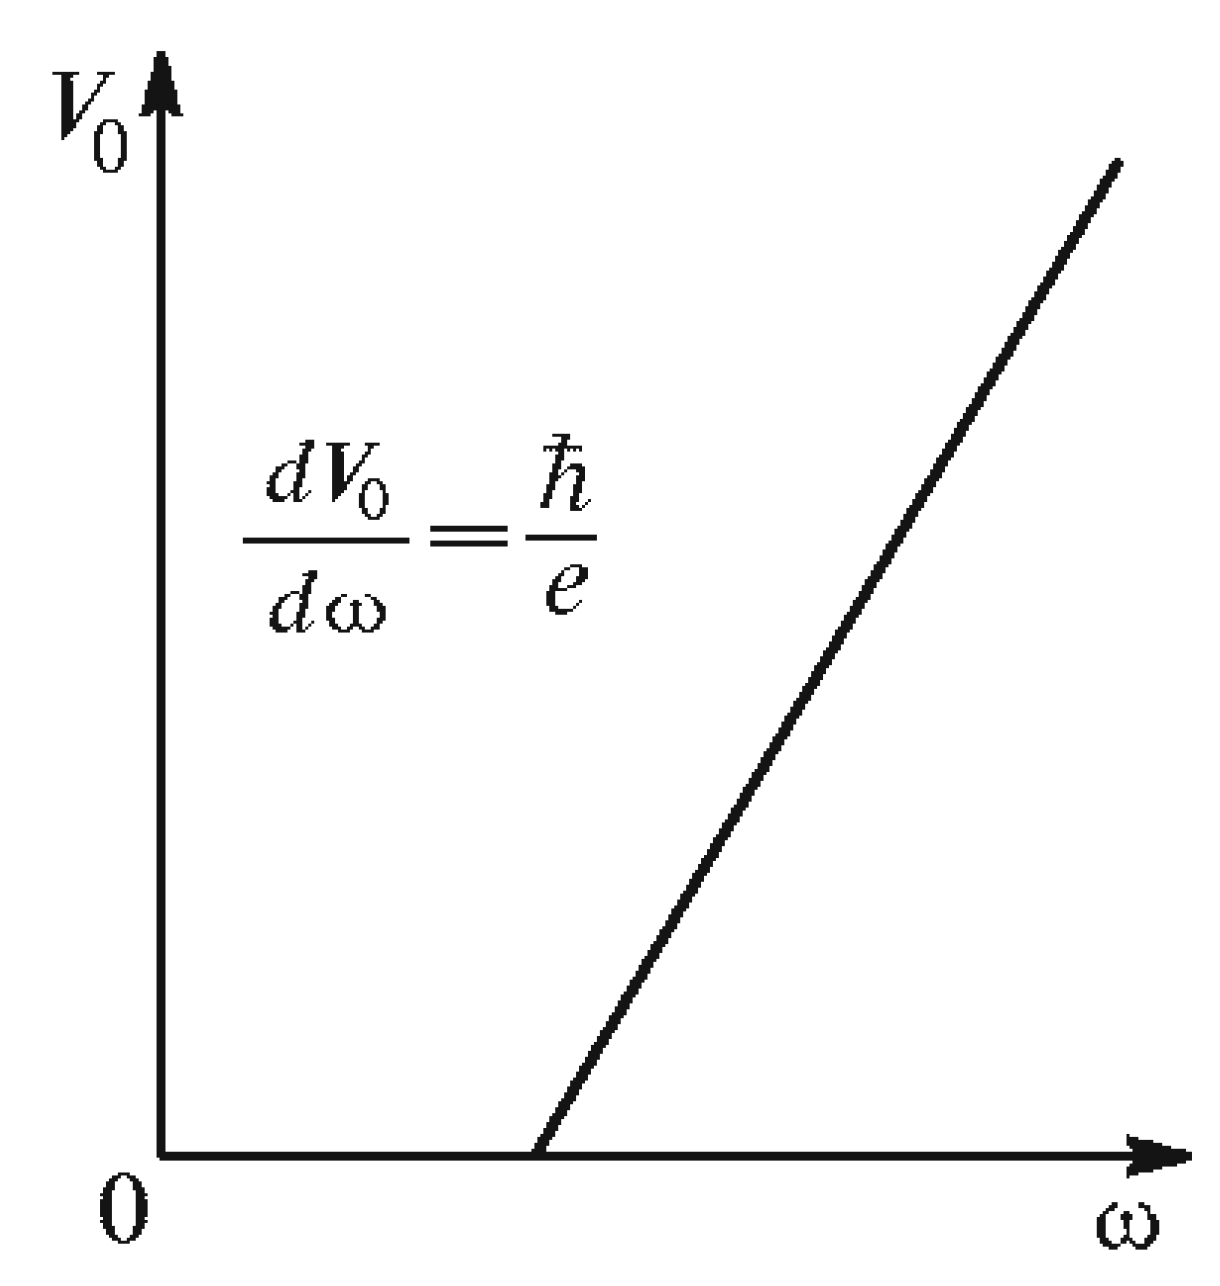
\includegraphics[width=\linewidth]{V(w)}
		\caption{Зависимость запирающего потенциала
			от частоты света}
		\label{ris V(w)}
	\end{wrapfigure}
	
	Потенциал запирания $ V_0 $ для любого катода линейно зависит от
	частоты света $ \omega $. По наклону прямой на графике $ V_0(\omega) $ (рис. \ref{ris V(w)}) можно определить постоянную Планка:
	
	\begin{equation}\label{dV/dw}
	\dfrac{dV_0}{d\omega} = \dfrac{\hbar}{e}
	\end{equation}
	
	Как показывает формула \eqref{dV/dw}, угол наклона прямой $ V_0(\omega) $ не зависит от рода вещества, из которого изготовлен фотокатод. От рода вещества, однако, зависит величина фототока, работа выхода $ W $ и форма кривой $ I(V) $ (рис. \ref{ris I(V)}). Все это определяет выбор пригодных для
	опыта катодов.

\section{Методика измерений}

Схема экспериментальной установки приведена на рис.~\ref{fig:ust}. Свет от
источника S (обычная электрическая лампа накаливания) с помощью
конденсора фокусируется на входную щель призменного монохроматора
УМ-2, выделяющего узкий спектральный интервал, и попадает на катод
фотоэлемента ФЭ.

\begin{figure}[h]
\begin{center}
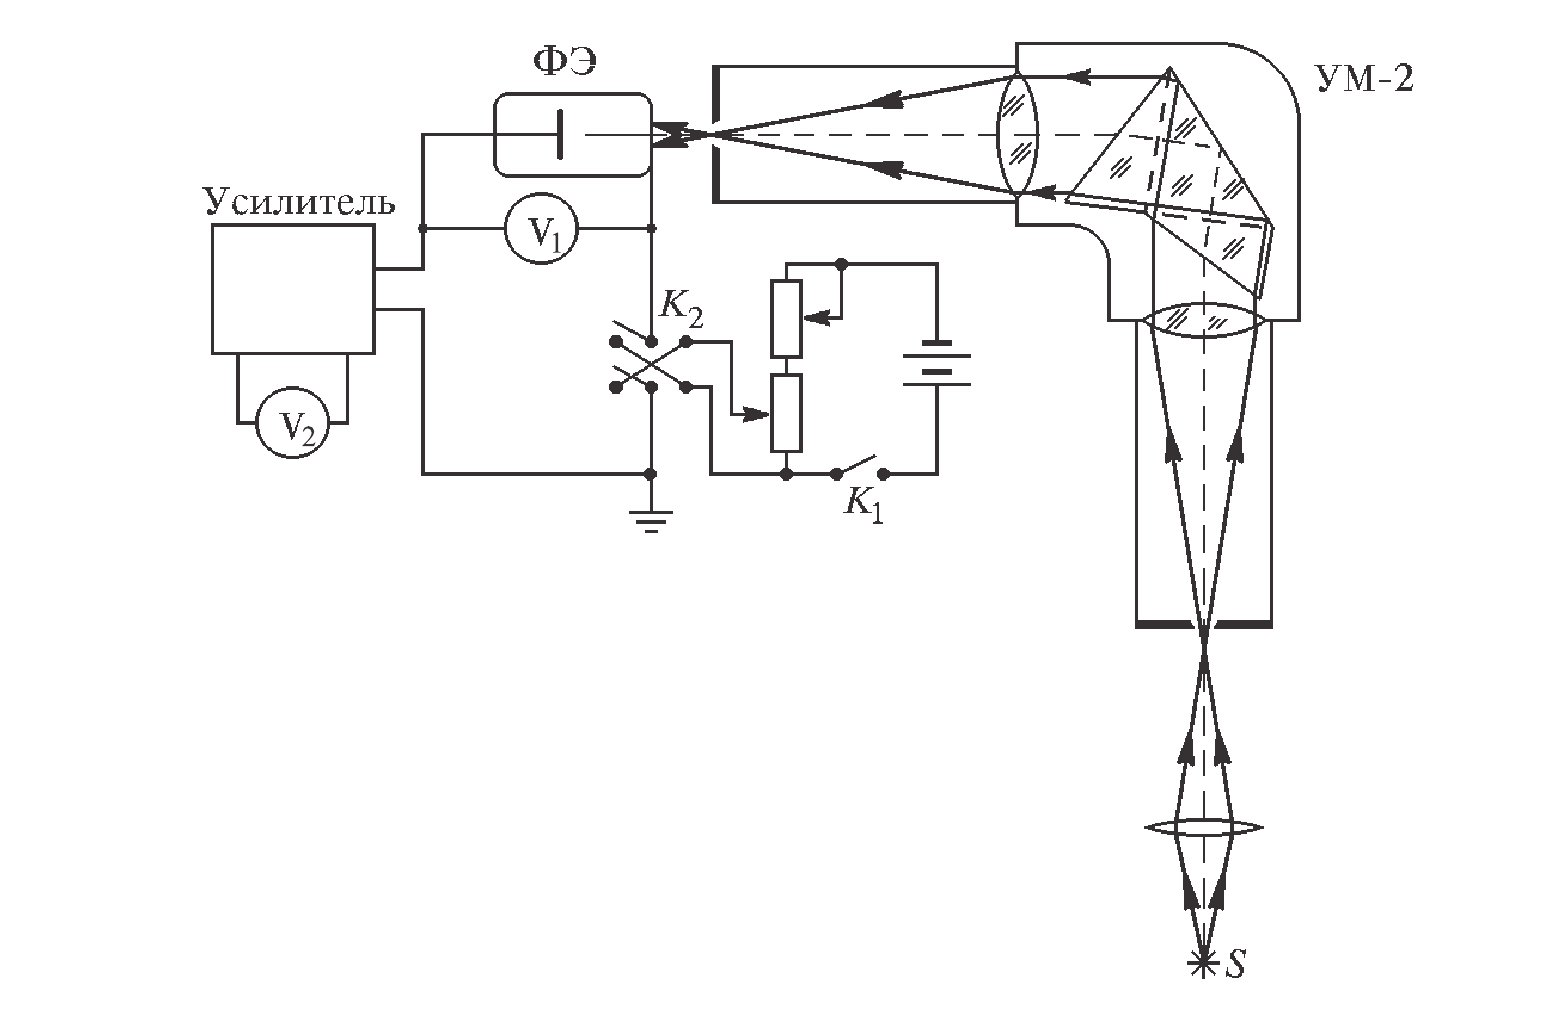
\includegraphics[width = \textwidth]{ust.png}
\caption{Принципиальная схема экспериментальной установки}
\label{fig:ust}
\end{center}
\end{figure}

Фотоэлемент конструктивно представляет собой откачанный до высокого вакуума стеклянный баллон диаметром 25 мм и высотой 30 мм.
Внутри баллона расположены два электрода: фотокатод и анод. Фотокатод представляет собой тонкую пленку металла, легированного элементами $Na$, $K$, $Sb$ и $Cs$ и расположенного на массивной металлической
пластине. Анод фотоэлемента выполнен в виде пояска тонкой пленки,
осажденной на внутренней части боковой поверхности вверху баллона.
Такое расположение фотокатода и анода обеспечивает наиболее полный
сбор на аноде электронов, эмитированных фотокатодом. Фотокатод и
анод имеют вплавленные в стекло колбы никелевые выводы для подключения к внешней схеме. Такой фотоэлемент обладает спектральной
чувствительностью в области длин волн от 300 до 850 нм. Наибольшая
чувствительность ФЭ лежит в области от 400 до 500 нм.

Фототок, протекающий в фотоэлементе, мал, особенно при потенциалах $V$ , близких к $V_0$, и не может быть измерен непосредственно. Для
его измерения используется усилитель постоянного тока. Для уменьшения погрешностей измерений, обусловленных наводками, усилитель
фототока смонтирован в одном корпусе с ФЭ. Абсолютные значения фототока нам не нужны, поэтому он измеряется в относительных единицах цифровым вольтметром $V_2$, подключенным к выходу усилителя.
Эти показания пропорциональны величине измеряемого тока. Тормозящий потенциал регулируется при помощи двух потенциометров «Грубо»
и «Плавно», установленных на корпусе блока питания установки. Измерение тормозящего потенциала осуществляется с помощью цифрового
вольтметра $V_1$.

Контактная разность потенциалов между катодом и анодом мешает
точному определению величины $V_0$, но не оказывает влияния на определение постоянной Планка, которая выражается через производную
$dV_0/d\omega$.

%\section{Используемое оборудование}
%
%\begin{enumerate}
%    \item компьютер;
%    \item источник излучения;
%    \item графитовая мишень;
%    \item счётчик $\gamma$-квантов;
%\end{enumerate}

\section{Результаты измерений и обработка данных}

Сначала выполним градуировку монохроматора. Проведем серию измерений для линий спектра неона, снимая зависимость длины волны света от параметра $ \theta $ барабана монохроматора. Построим графики зависимости, аппроксимируя функцию $ \lambda (\theta) $ многочленом второй степени в силу нелинейности. Градуировочный график представлен на рис.~\ref{plot:calibr}.

\begin{figure}[h]
\begin{center}
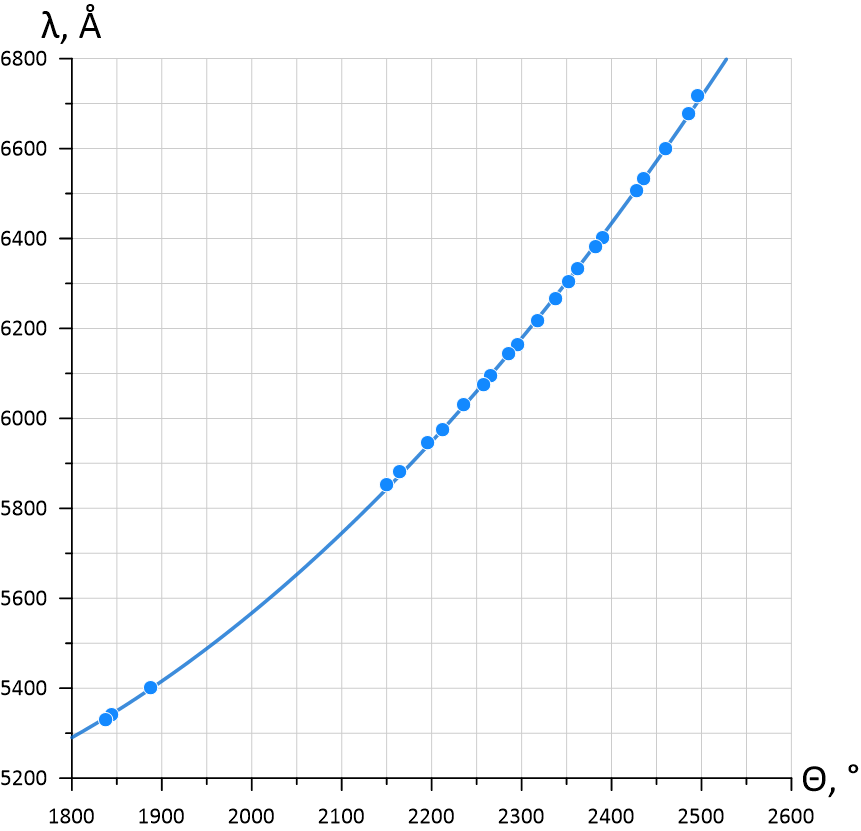
\includegraphics[width = 0.8\textwidth]{calibr.png}
\caption{Градуировочная кривая}
\label{plot:calibr}
\end{center}
\end{figure}

Теперь проведем 6 серий измерений зависимости фототока от напряжения для разных длин волн падающего света, изменяя на монохроматоре параметр $ \theta $ и переводя его в длину волны с помощью градуировки.
	
Результаты измерений представлены на рис.~\ref{fig:purp}-\ref{fig:red}. Согласно формуле \eqref{sqrt I = V}, построим графики зависимости в координатах $ \sqrt{I} (V) $ и аппроксимируем линейные участки прямой. Экстраполируя прямую к нулю, получим значения потенциала запирания для каждой серии измерения (длины волны). Результаты представлены в таб.~\ref{tab:V}.

\begin{figure}[h]
\begin{center}
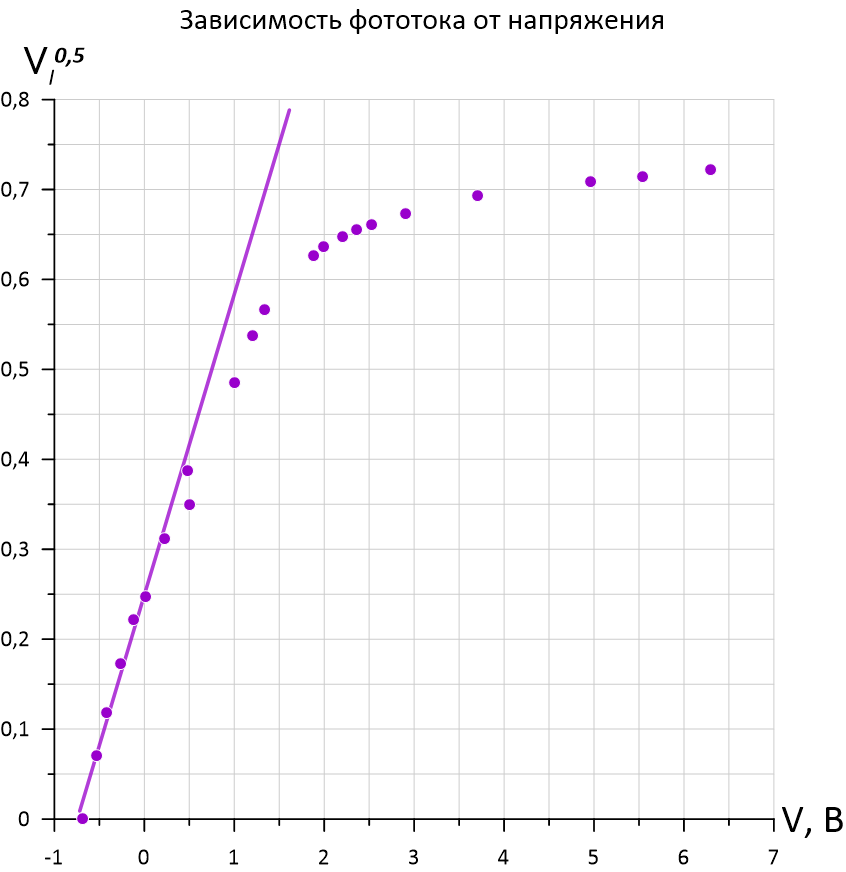
\includegraphics[width = 0.5\textwidth]{5401.png}
\caption{$\lambda = 5401 \mathring{A}$}
\label{fig:purp}
\end{center}
\end{figure}

\begin{figure}[h]
\begin{center}
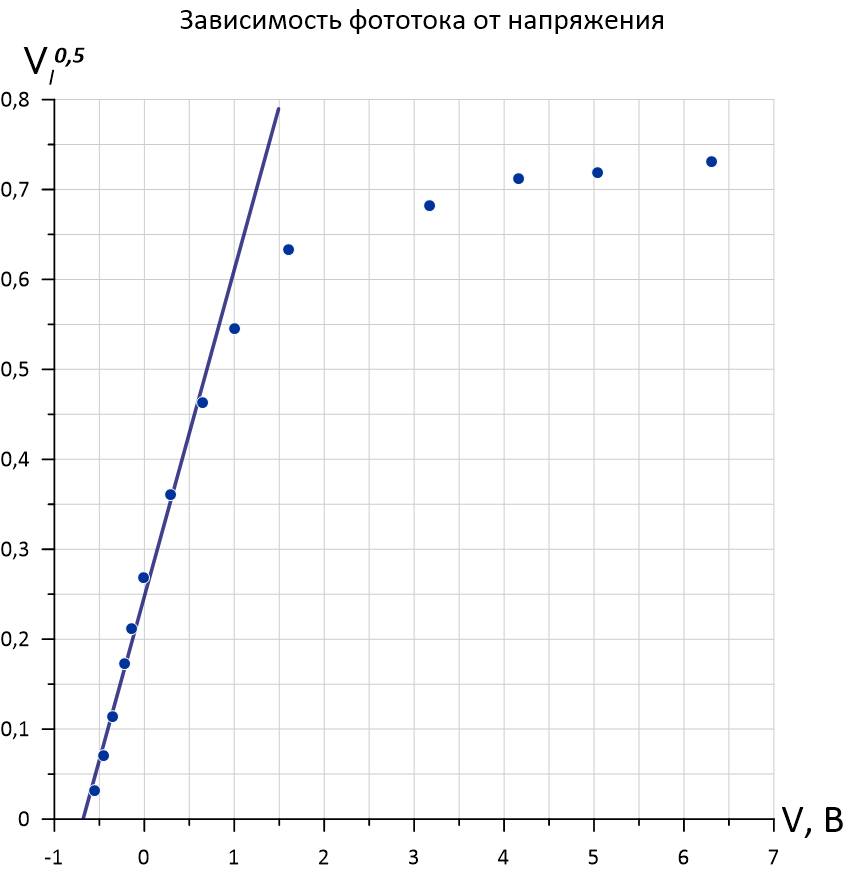
\includegraphics[width = 0.5\textwidth]{5945.png}
\caption{$\lambda = 5945 \mathring{A}$}
\label{fig:blue}
\end{center}
\end{figure}

\begin{figure}[h]
\begin{center}
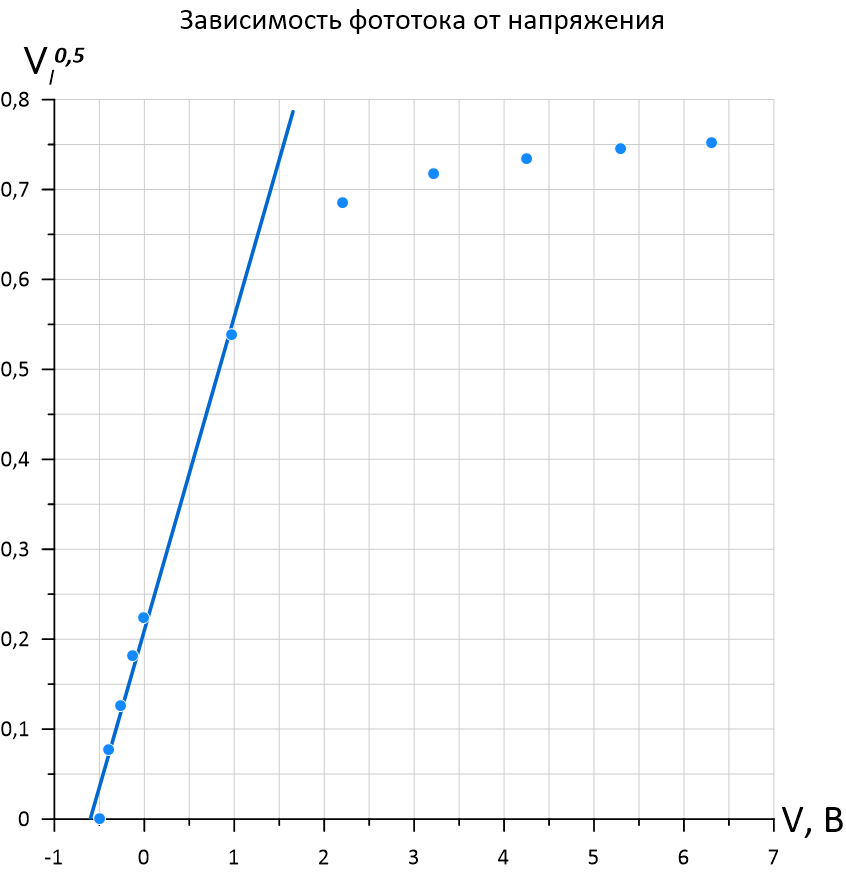
\includegraphics[width = 0.5\textwidth]{6074.png}
\caption{$\lambda = 6074 \mathring{A}$}
\label{fig:cyan}
\end{center}
\end{figure}

\begin{figure}[h]
\begin{center}
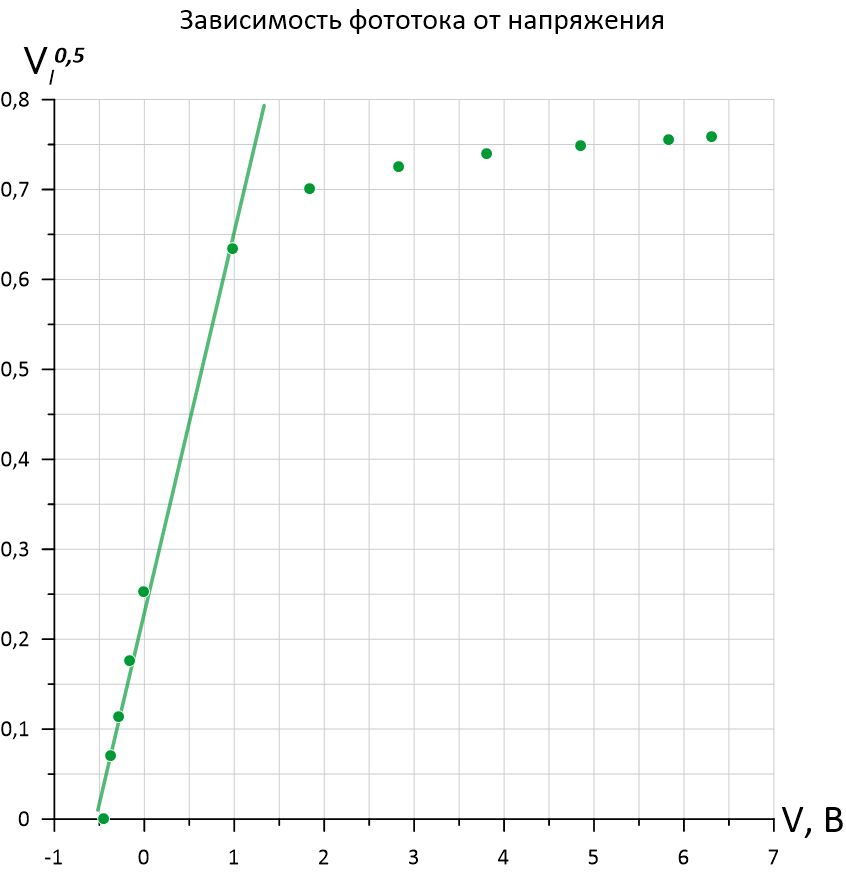
\includegraphics[width = 0.5\textwidth]{6267.png}
\caption{$\lambda = 6267 \mathring{A}$}
\label{fig:green}
\end{center}
\end{figure}

\begin{figure}[h]
\begin{center}
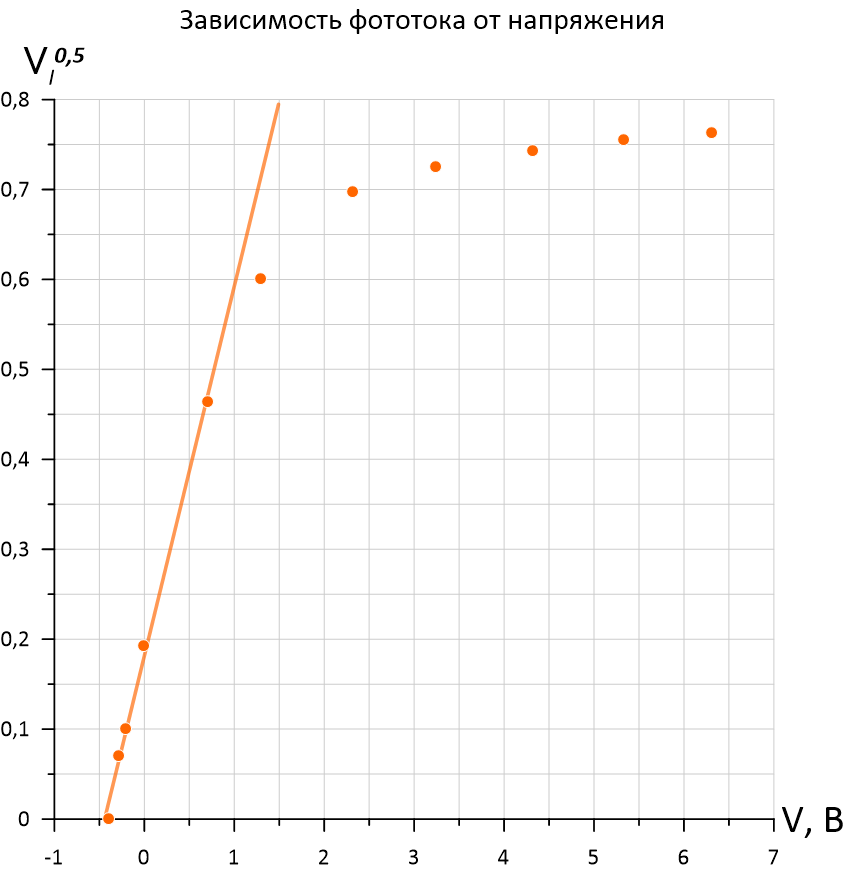
\includegraphics[width = 0.5\textwidth]{6533.png}
\caption{$\lambda = 6533 \mathring{A}$}
\label{fig:oran}
\end{center}
\end{figure}

\begin{figure}[h]
\begin{center}
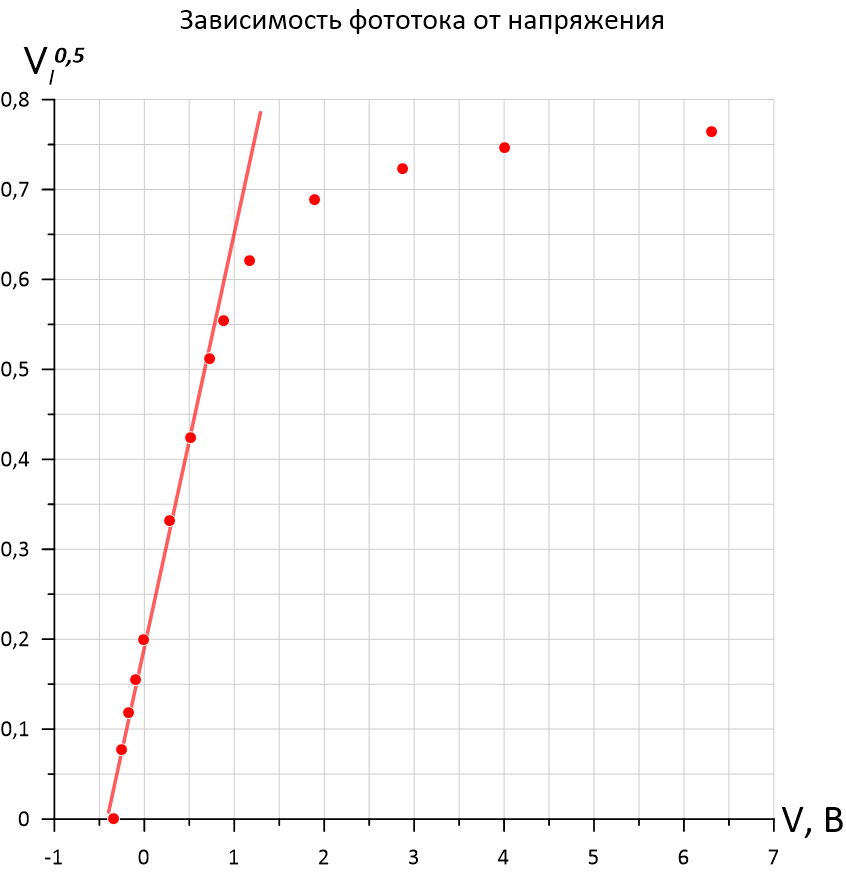
\includegraphics[width = 0.5\textwidth]{6717.png}
\caption{$\lambda = 6717 \mathring{A}$}
\label{fig:red}
\end{center}
\end{figure}

\begin{table}[h!]
	\begin{center}
			\begin{tabular}{|c|c|c|c|}
			\hline
			$\lambda$, \AA & a & b & $-V_0$, B \\ 
			\hline 
			5401 & 0.334 & 0.249 & $0.745\pm0.074$ \\ 
			\hline 
			5945 & 0.363 & 0.247 & $0.681\pm0.068$ \\ 
			\hline 
			6074 & 0.348 & 0.209 & $0.601\pm0.060$ \\ 
			\hline 
			5267 & 0.423 & 0.229 & $0.541\pm0.054$ \\ 
			\hline 
			6533 & 0.410 & 0.181 & $0.441\pm0.044$ \\ 
			\hline
			6717 & 0.460 & 0.190 & $0.413\pm0.041$ \\ 
			\hline  
			\end{tabular} 
	\end{center}
	\caption{Параметры линейной аппроксимации для различных длин волн и запирающее напряжение} 
	\label{tab:V}
\end{table}

Теперь построим график зависимости $ V_0(\omega) $. Согласно \eqref{V(w)} аппроксимируем прямой.

\begin{figure}[h]
\begin{center}
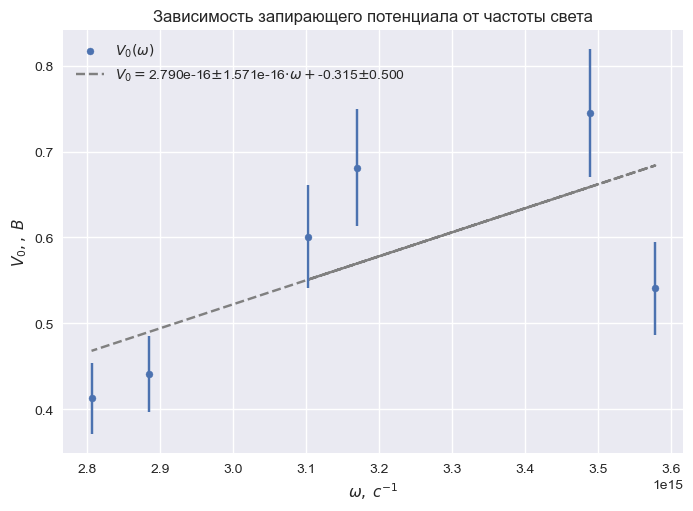
\includegraphics[width = 0.8\textwidth]{V0(w).png}
\caption{График зависимость запирающего напряжения от частоты излучения}
\label{fig:V0(w)}
\end{center}
\end{figure}

Из наклона прямой согласно \eqref{dV/dw} получаем значение постоянной Планка:
	
	\begin{equation}\label{}
	\frac{dV_0}{d\omega} = \frac{\hbar}{e} \Rightarrow \hbar = 2,79 \cdot 10^{-16} \cdot 1,602 \cdot 10^{-19} \approx (0,447 \pm 0,251) \cdot 10^{-34} \; Дж \cdot с 
	\end{equation}
	
\section{Обсуждение результатов и выводы}

Таким образом, в ходе выполнения работы мы убедились в явлении фотоэффекта и с помощью уравнения Эйнштейна измерили постоянную Планка. Полученное значение:
\begin{equation}
\boxed{\hbar = (0,447 \pm 0,251) \cdot 10^{-34} \; Дж \cdot с}
\end{equation}
Табличное значение: $ \hbar = 1,054 \cdot 10^{-34} \; Дж \cdot с $. Полученный результаты близок к табличному значению. 

\end{document}
